\chapter{Konzept} \label{chap:konzept}
In diesem Kapitel wird zunächst erläutert, wie die Steuerung der Getränkemischmaschine durch Sprachbefehle im Allgemeinen ablaufen wird.
Anschließend werden mehrere Konzepte vorgestellt, die das allgemeine Konzept konkretisieren.
Diese werden anhand der, in Kapitel \ref{section:Bewertungskriterien} erläuterten Kriterien, bewertet.
Zuletzt wird die Wahl des finalen Konzepts begründet.
\section{Allgemein}
Der Benutzer soll über Spracheingaben mit der Mischmaschine interagieren können.
Dafür muss das Gesprochene zunächst durch ein Mikrofon aufgenommen werden.
Anschließend können die Audiosignale weiterverarbeitet werden.
Der Benutzer soll hierbei nicht auf fest vorgegebene Sprachbefehle beschränkt sein, sondern für nahezu jede Eingabe eine sinnvolle Antwort zurückerhalten.
Um dies zu gewährleisten wird die Spracheingabe durch ein Sprachmodell, welches mittels maschinellen Lernverfahren trainiert wurde, verarbeitet.
Ergebnisse dieser Verarbeitung sind die Antwort, die an den Benutzer zurückgegeben wird, und ein konkreter Befehl für die Mischmaschine.
Ein Beispiel für einen solchen Befehl könnte etwa die Zubereitung eines bestimmten Getränks sein.
Für die Ausgabe einer Antwort ist ein Lautsprecher notwendig.
Denkbar wäre auch eine textbasierte Ausgabe, allerdings ginge damit der Eindruck des Benutzers verloren eine echte Konversation mit der Mischmaschine zu führen.
Das Sprachmodell mit der Getränkemischmaschine zu verknüpfen stellt eine Herausforderung dieser Arbeit dar.
\section{Bewertungskriterien} \label{section:Bewertungskriterien}
Im Folgenden sind die Bewertungskriterien für die einzelnen Konzepte aufgelistet:
\begin{itemize}
    \item Freiheitsgrade in der Spracheingabe des Benutzers: Erhält der Benutzer passende Antworten zurück egal was er sagt oder ist er auf einige wenige Befehle beschränkt?
    \item Hardwarekosten: Wie kostspielig ist das Konzept bezüglich der zusätzlich benötigten Hardware?
    \item Verfügbare Rechenleistung: Wie hoch ist die Verfügbare Rechenleistung im Vergleich zu den anderen Konzepten? Reicht diese aus um das Sprachmodell auszuführen?
    \item Performanz: Als wie performant wird die Lösung eingeschätzt? Ist mit Latenzen zwischen der Einagbe des Benutzers, der Ausgabe einer Antwort und Ausführung der Aktion zu rechnen?
    \item Overhead: Wie hoch ist im Allgemeinen der Mehraufwand einzuschätzen?
\end{itemize}
\section{Konzept A: Spracherkennung und -verarbeitung mittels Arduino} \label{section:Konzept_A}
Ein erstes Konzept sieht vor, dass das Audiosignal direkt von einem der Arduinos in der Getränkemischmaschine aufgenommen wird.
Das Audiosignal wird vom Arduino interpretiert und eine passende Antwort wird ausgegeben.
Außerdem sendet der Arduino die entsprechenden Signale, um die vom Benutzer gewünschte Aktion von der Getränkemischmaschine ausführen zu lassen.
Ein Problem ist hierbei die Interpretation des Audiosignals durch den Arduino, da dessen Leistung nicht für das Ausführen eines Sprachmodells ausreicht.
Folglich muss dieser Prozess ausgelagert werden.
Das Konzept wird deshalb um ein cloudbasiertes Sprachverarbeitungssystem ergänzt, welches den Sprachbefehl des Benutzers vom Arduino entgegennimmt und einen passenden Befehl und eine passende Antwort zurückgibt (s. Abb. \ref{figure:Spracherkennung_mittels_Arduino}).
Die Kommunikation zwischen Arduino und Cloudsystem kann über das \ac{HTTP} erfolgen.
\begin{figure}[H]
    \centering
    % \includegraphics does not allow jpg images apparently!
    \fbox{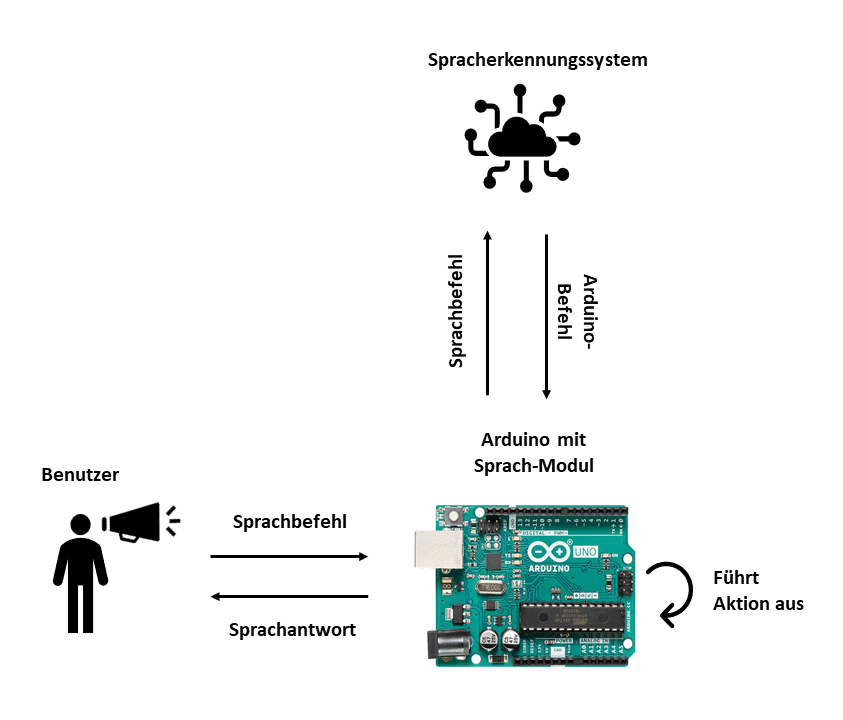
\includegraphics[width=0.8\textwidth]{Bilder_Kapitel_3/Konzept_A.png}}
    \caption{\label{figure:Spracherkennung_mittels_Arduino}Spracherkennung und -verarbeitung mittels Arduino}
\end{figure}
\noindent
Es muss ein geeignetes Format zum Versenden des Sprachbefehls über \ac{HTTP} gefunden werden.
Eine Möglichkeit besteht darin, das eingehende Audiosignal im Arduino in textform umzuwandeln und diesen String zu versenden.
Die auf dem Markt verfügbaren Arduino-Sprach-Module sind jedoch nicht in der Lage beliebige Spracheingaben in Text umzuwandeln, sondern bieten diese Funktionalität nur für vordefinierte Werte an.
Dies würde das Ziel dieser Arbeit verfehlen, dem Benutzer eine Konversation mit der Mischmaschine zu ermöglichen.
Ein weiteres Problem dieser Lösung besteht darin, dass beispielsweise bei wechselnder Getränkeauswahl die zur Verfügung stehenden Sprachbefehle wie "`Ich hätte gerne Getränk xy"' jedes Mal aufs neue manuell angepasst werden müssten.
Dies hat zur Folge, dass auch die reine Spracherkennung aus der Mischmaschine ausgelagert werden muss.
Ein denkbares Format sind die rohen Audiosignale, die vom Arduino aufgenommen werden.
\section{Konzept B: Spracherkennung und -verarbeitung mittels mobiler Anwendung}
Die Audiosignale über ein Mikrofon in der Mischmaschine aufzunehmen und eine Antwort über einen Lautsprecher auszugeben, so wie es in Konzept A der Fall ist, kann ein Problem darstellen.
Zum Einen wird dadurch zusätzliche Hardware benötigt und zum Anderen muss diese korrekt verbaut werden.
Das Tonsignal muss vom Mikrofon in einer guten Qualität aufgenommen werden können und die Antwort aus dem Lautsprecher für den Benutzer verständlich sein.
Konzept B umgeht dieses Problem durch den Einsatz einer mobilen Anwendung, die durch den Benutzer installiert wird.
Über diese Anwendung können anschließend die Aufnahme der Audiosignale, die Spracherkennung und die Kommunikation mit dem Sprachverarbeitungsservice und der Mischmaschine abgewickelt werden, wie in Abbildung \ref{figure:Konzept_mobile_App} zu sehen ist.
\begin{figure}[H]
    \centering
    \fbox{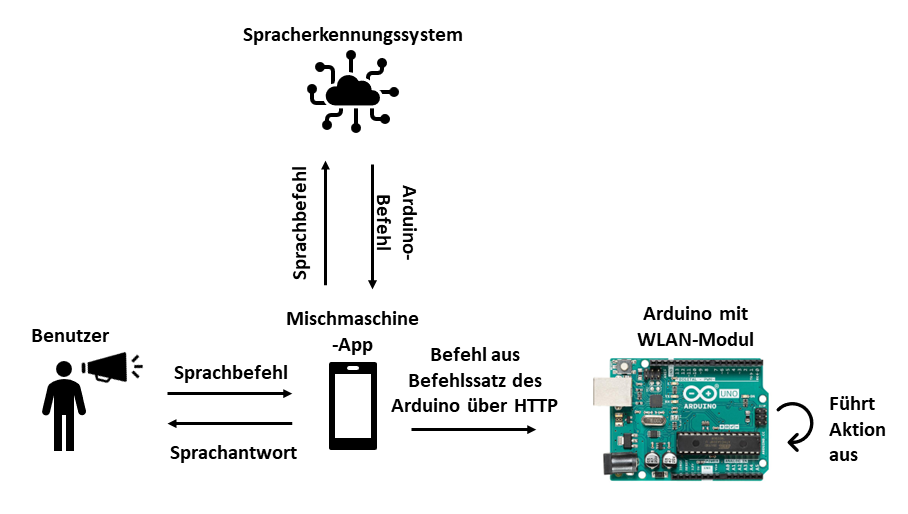
\includegraphics[width=0.8\textwidth]{Bilder_Kapitel_3/Konzept_B.png}}
    \caption{\label{figure:Konzept_mobile_App}Spracherkennung und -verarbeitung mittels mobiler Anwendung}
\end{figure}
\noindent
Ein Problem dieser Lösung ist der offensichtliche Mehraufwand durch die Entwicklung einer eigenen Anwendung für Mobiltelefone.
Auch der Anwender hat zusätzlichen Aufwand durch die Installation.
Außerdem ist die Spracheingabe und -ausgabe über das Mobiltelefon nicht intuitiv, da der Anwender eigentlich mit der Maschine kommunizieren sollte.
Dieser Effekt kann dadurch abgeschwächt werden, dass wenigstens die Antwort durch einen Lautsprecher in der Mischmaschine an den Benutzer zurückgegeben wird.
\section{Konzept C: Spracherkennung und -verarbeitung auf Computer-Hardware}
Ein weiteres Konzept stützt sich auf die Verwendung eines Computers in der Mischmaschine anstelle eines Mikrocontrollers wie dem Arduino.
Motivation ist hierbei der Leistungsgewinn gegenüber eines Mikrocontrollers, um die Spracherkennung und -verarbeitung mittels Sprachmodell zu gewährleisten.
Ein Beispiel für einen solchen Miniaturcomputer ist der Raspberry-Pi.
Dieser bietet genügend Schnittstellen, wie etwa USB-Hubs, zum verbinden von Mikrofon als auch Lautsprecher.
Nimmt der Computer das Audiosignal auf verarbeitet er dieses und generiert daraus die Antwort, die durch den Lautsprecher ausgegeben wird, zusammen mit der Aktion für die Getränkemischmaschine.
Diese muss an den Arduino, welcher die Mischmaschine steuert, übermittelt werden.
Um dies zu ermöglichen können der Computer und der Arduino über eine serielle Schnittstelle, wie etwa einem USB-Kabel, miteinander  verbunden werden.
Abbildung \ref{figure:Konzept_Raspberry} stellt den konzeptionellen Aufbau graphisch dar.
\begin{figure}[H]
    \centering
    \fbox{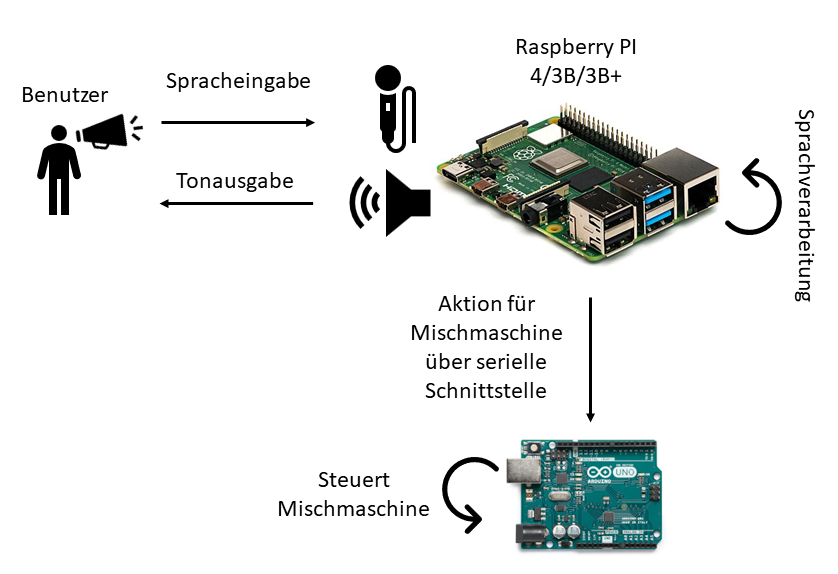
\includegraphics[width=0.8\textwidth]{Bilder_Kapitel_3/Konzept_C.png}}
    \caption{\label{figure:Konzept_Raspberry}Spracherkennung und -verarbeitung auf Computer-Hardware}
\end{figure}
\noindent
Obwohl ein Computer wie der Raspberry-Pi im Allgemeinen eine höhere Leistung als ein Mikrocontroller hat ist damit nicht sichergestellt, dass diese zur Ausführung des Sprachmodells ausreicht.
Beispielsweise ist das vierte Modell der Raspberry-Pi-Serie mit nur maximal acht Gigabyte Arbeitsspeicher erhältlich.
Das Sprachmodell könnte allerdings noch weitaus mehr Daten im Arbeitsspeicher benötigen.
Des Weiteren ist zu beachten, dass die Miniaturcomputer von Raspberry-Pi im Speziellen zum Zeitpunkt dieser Arbeit kaum zu vertretbaren Preisen verfügbar sind.
\section{Konzept für die Sprachsteuerung}
\subsection{Ansatz für das Dialogsystem}
Aus dem Vergleich der wichtigsten Ansätze zur Erstellung von Chatbots, die in Kapitel \ref{sec:ansaetze_erstellung_chatbots} besprochen wurden, lassen sich die folgenden Vor- und Nachteile der einzelnen Methoden ableiten:
\begin{table}[H]
    \centering
    \begin{tabular}{m{3cm}|m{6cm}|m{6cm}}
        Ansatz               & Vorteile                                                  & Nachteile \\
        \hline
        Musterabgleich       & \makecell[l]{\tabitem Einfacher Einstieg                              \\ \tabitem Leicht wiederverwendbar\\ \tabitem Modularität\\ \tabitem Leicht zu kontrollieren/\\einzuschränken} & \makecell[l]{\tabitem Themenbereich begrenzt\\ \tabitem Die Möglichkeiten sind durch\\ die Arbeitsbelastung des\\ Entwicklers begrenzt\\ \tabitem Komplexität der Fehlersuche\\ \tabitem Strenge und \glqq{}spröde\grqq{} Regeln} \\
        \hline
        Grounding            & \makecell[l]{\tabitem Gut im Beantworten logischer\\ Fragen             \\\tabitem Leicht zu kontrollieren/\\einzuschränken}             & \makecell[l]{\tabitem Künstlicher, mechanischer Ton \\ \tabitem Probleme mit Zweideutigkeiten \\ \tabitem Probleme mit dem Allgemein-\\wissen \\ \tabitem Begrenzt auf strukturierte\\ Daten \\ \tabitem Erfordert die Extraktion von\\ Informationen in großem Umfang \\ \tabitem Erfordert menschliche Aufsicht}    \\
        \hline
        Suche                & \makecell[l]{\tabitem Einfachheit                                     \\ \tabitem Leicht zu lehren \\ \tabitem Simulation von menschlicher\\ Konversation}             & \makecell[l]{\tabitem Unzureichende Skalierung \\ \tabitem Die simulierte Persönlichkeit des\\ Bots ist inkonsistent \\ \tabitem Kennt den Kontext nicht \\ \tabitem Keine sachlichen Fragen} \\
        \hline
        \makecell[l]{Generierungs-\\methoden} & \makecell[l]{\tabitem Neue, kreative Dialoge                          \\ \tabitem Weniger Arbeit für den\\ Entwickler \\ \tabitem Kontextsensitiv}           & \makecell[l]{\tabitem Schwierig zu lehren \\ \tabitem Erfordert mehr Daten (Dialoge) \\ \tabitem Schwierig, in die richtige\\ Richtung zu lenken \\ \tabitem Erfordert mehr Rechenleistung} \\
    \end{tabular}
    \caption{\label{table:Bewertungsmatrix_Konzepte_Dialogsysteme}Bewertung der Ansätze für die Erstellung eines Dialogsystems}
\end{table}
\noindent
Bei der Analyse des Problems, ein Dialogsystem für eine Getränkmischmaschine zu entwickeln, kann man zu dem Schluss kommen, dass die beste Option eine Mischung aus dem Ansatz der Informationssuchemethode und dem Musterabgleich ist.\\\\
Das erste Argument, das für diesen Ansatz spricht, ist die Möglichkeit, die Sprachsteuerung in deutscher Sprache zu verwenden, was die Anwendung der Generierungsmethoden erschwert, da der Zugang zu einer geeigneten Datenbank in dieser Sprache, die den Anforderungen des Projekts, nämlich eine ausreichende Anzahl von Beleidigungen zu enthalten, nicht möglich ist.
Gleichzeitig können bei der Verwendung von Musterabgleich Antwortvorlagen und Muster für entsprechende Anfragen in deutscher Sprache im Voraus erstellt werden, was die Erstellung und das Training des Dialogsystems erleichtert.\\\\
Das zweite Argument ist, dass in diesem Projekt ein Raspberry Pi verwendet wird, was die Verwendung generativer Methoden aufgrund der begrenzten Hardware-Ressourcen einschränken kann.
Andererseits kann das Modell für die Informationssuche und den Musterabgleich auf Geräten mit geringem Stromverbrauch implementiert werden, was diesen Ansatz für dieses Projekt vorteilhaft macht.\\\\
Generierungsmethoden könnten auch für dieses Problem zu mächtig sein.
Beim Mixen von Cocktails können die Antworten einfach und formelhaft sein, wie z. B. \glqq{}Das hört sich eklig an, bist du sicher, dass du es willst?\grqq{} oder \glqq{}Ich hoffe, ich sehe dich nie wieder\grqq{}.
In diesem Fall kann der Einsatz von Generierungsmethoden wie seq2seq-Modellen überflüssig und ineffizient sein.
Für diese Aufgabe ist im Gegensatz zu komplexen natürlichsprachlichen Abfragen keine detaillierte semantische Verarbeitung erforderlich, so dass der Musterabgleich einen einfacheren und effizienteren Ansatz darstellt.\\\\
Bei der Verwendung des Musterabgleiches kann man den Ton und den Humor des Geräts leicht steuern und so die gewünschte Atmosphäre erzeugen.
Die Antworten des seq2seq-Modells sind wiederum sehr schwer zu steuern.
Generierungsmethoden können zu unerwünschtem Maschinenverhalten führen, wenn das Modell auf ungeeigneten Daten trainiert wird oder Fehler in der Betriebslogik enthält.
Die Verwendung einer Datenbank, die genügend Beleidigungen enthält (z. B. die 4chan-Datenbank), kann dazu führen, dass die Antworten der Maschine über das Ziel hinausschießen und statt lustig zu sein, den Benutzer beleidigen.\\\\
Mit diesem Ansatz wird auch die Effizienz der Maschinensteuerung verbessert.
Beim Musterabgleich kann eine Kategorie \glqq{}Getränkebestellung\grqq{} zugewiesen werden, die, wenn sie erkannt wird, die Maschine automatisch zur Bearbeitung der Befehle veranlasst.
Im Falle von seq2seq-Modell ist keine Kategorie vorgesehen, so dass eine zusätzliche Prüfung jeder Eingabeanweisung eingeführt werden müsste, um festzustellen, wann der Benutzer die Bestellung aufgegeben hat.\\\\
Ein letztes Argument, das für den Ansatz spricht, ist die Möglichkeit, die Maschine bei Bedarf schnell an neue Anfragen und Anforderungen anzupassen, indem neue Muster und Regeln in das System eingeführt werden.
Daher ist eine Mischung aus Informationssuchemethode und Musterabgleich für das vorliegende Problem am besten geeignet.
\subsection{Befehle}
\section{Finales Konzept}
Die folgende Tabelle zeigt eine Übersicht bezüglich der Bewertung der einzelnen Konzepte.
\begin{table}[H]
    \centering
    \begin{tabular}{l|c|c|c|c}
        Bewertungsmatrix          & \makecell{Konzept A                                     \\ (nur Arduino)} & Konzept A & Konzept B & Konzept C \\
        \hline
        \makecell[l]{Freiheitsgrade in der Spracheingabe                                    \\ des Benutzers} & niedrig                    & sehr hoch & sehr hoch & hoch      \\
        \hline
        Hardwarekosten            & niedrig             & hoch      & niedrig   & sehr hoch \\
        \hline
        Verfügbare Rechenleistung & niedrig             & sehr hoch & sehr hoch & hoch      \\
        \hline
        Performanz                & sehr hoch           & mittel    & mittel    & sehr hoch \\
        \hline
        Overhead                  & niedrig             & hoch      & sehr hoch & niedrig   \\
    \end{tabular}
    \caption{\label{table:Bewertungsmatrix_Konzepte}Bewertung der Konzepte}
\end{table}
\noindent
Ein erster Ansatz wurde im Kapitel \ref{section:Konzept_A} zu Konzept A erläutert.
Hierbei war die Idee, die Spracherkennung und -verarbeitung nur auf dem Arduino auszuführen.
Aufgrund der mangelnden Leistung eines Arduinos können mit Hilfe von Sprachmodulen jedoch nur vordefinierte Sätze oder Wörter erkannt werden.
Damit ist der Freiheitsgrad in der Spracheingabe des Benutzers äußerst eingeschränkt.
Dafür sind die aufzuwendenden Hardwarekosten minimal.
Lediglich das Sprachmodul sowie ein Lautsprecher müssten besorgt werden.
Die Performanz wird als sehr hoch eingeschätzt, da die Spracherkennung direkt auf dem Ardunino erfolgen kann, der auch die Mischmaschine steuert.
Niedrig ist hingegen der benötigte Mehraufwand, da kaum zusätzliche Awendungen, Services oder Hardwarekomponenten benötigt werden.\\\\
Das Konzept wurde schließlich durch einen Sprachverarbeitungsservice in der Cloud ergänzt (Konzept A).
Der Benutzer hat bei diesem Ansatz große Freiheiten in seinen Formulierungen, da es kein Problem darstellt ein großes Sprachmodell in der Cloud auszuführen.
Die Hardwarekosten könnten allerdings hoch sein, je nach dem, ob der Server selbst bereitgestellt oder von einem externen Anbieter bezogen wird.
Auch die letzten Endes tatsächlich benötigte Rechenleistung spielt dabei eine Rolle.
Die verfügbare Rechenleistung ist theoretisch unbegrenzt, wobei die Performanz des Gesamtsystems nur als mittelmäßig eingestuft werden kann.
Nach der Aufnahme und eventuell einer Vorverarbeitung des Aduiosignals durch den Arduino müssen \ac{HTTP}-Nachrichten gesendet und Empfangen werden.
Je nach Last auf dem Netzwerk kann es dadurch zu Latenzen oder sogar Verbindungsabbrüchen kommen.
Außerdem ist der Overhead durch den Einsatz einer Cloud recht hoch.\\\\
Konzept B unterscheidet sich in Sachen Freiheitsgrad, Rechenleistung und Performanz nicht von Konzept A, da auch hier eine Cloud zum Einsatz kommt.
Die Hardwarekosten sind jedoch niedriger, da immerhin kein Sprachmodul, Mikrofon und Lautsprecher benötigt werden.
Die Aufgaben dieser Komponenten kann das Mobiltelefon des Anwenders übernehmen.
Der Overhead ist deutlich größer, das das Konzept die Entwicklung einer eigenen Mobilanwendung voraussetzt.\\\\
Der Freiheitsgrad wird bei Konzept C als hoch, jedoch nicht als sehr hoch, bewertet.
Grund hierfür ist die, im Vergleich zur Cloud, etwas beschränkte Leistung, welche die Leistung/Größe des Sprachmodells beeinträchtigen könnte.
Hardwarekosten können jedoch sehr hoch werden.
Bei dem Einsatz einer Cloud kann ein günstiger Anbieter gefunden werden, sodass die Anschaffung eigener Hardware entfällt.
Dies ist hier nicht der Fall.
Die Performanz des Gesamtsystems kann, wie bei Konzept A (nur mittels Arduino), sehr hoch eingeschätzt werden, da Spracherkennung und -verarbeitung direkt in der Mischmaschine von der Hardware übernommen wird.
Der Mehraufwand ist gering, da weder ein Cloudservice noch eine externe Anwendung entwickelt werden müssen.
\endinput



